\usetikzlibrary{shapes.geometric}
\usetikzlibrary{positioning}

\newcommand{\apparatus}[4]{\node[square node] (#1) at (#2,#3){#4};
                           \node[port] (#1+) at (#2 + 0.375, #3 + 0.5){+};
                           \node[port] (#1-) at (#2 + 0.375, #3 - 0.5){-};}

\chapter{Stern-Gerlach Experiments}
TODO: provide a brief explanation of the experimental setup and results. Discuss historical and pedagogical significance. This section is background information so that I can discuss the von Neumann measurement, consistent histories, and decoherence in the context of this experiment. I am saving it for later to focus on the introducing the new theory for now.

\chapter{Postulates of Quantum Mechanics}

We first consider the mathematical objects used to model physical systems and variables. By comparing the objects used in classical and quantum mechanics, we make sense of the first three postulates of quantum mechanics. Then, we compare the Copenhagen and von Neumann descriptions of measurement and their relation to the fourth and fifth postulates.

\section{Physical Variables and State Spaces}
\subsection{Classical States}
Consider the spin of an electron. Treating the electron as a classical system, its spin state is modeled by a vector $S \in \mathbb{R}^3$:
\begin{align}
S = (S_x, S_y, S_z)
\end{align}

Each component $S_{x_i}$ is a physical variable representing the magnitude of spin oriented in the $\hat{x_i}$ direction.

$S$ has the capacity to determine spin in any direction using the inner product of the state space $\mathbb{R}^3$:
\begin{align}
S_n(S) = S \cdot \hat{n}
\end{align}

We see that in classical mechanics, physical variables are modeled using functions. Each function $S_n$ maps a spin state $S$ to a real scalar representing the spin of the electron aligned along the $\hat{n}$ axis.

What makes classial mechanics more familiar to everyday experience boils down to intuitive but important properties of the state space $\mathbb{R}^3$:
\begin{itemize}
\item For any direction $\hat{n}$, $S$ determines spin $S_n$
\item $S_n$ can be any real value
\end{itemize}

$S$ determines spin in any direction because TODO. Consequently, the sample spaces for spin in any two directions $\hat{n}$ and $\hat{m}$ are \textit{compatible}, meaning that $S_n$ and $S_m$ may be simultaneously determined. Spin states in $\mathbb{R}^3$ are interpreted physically as the electron posessing definite values for every $S_n$ at some instant in time.

In addition to spin states determing all $S_n$, the state space allows $S_n$ to take on any real value. There are no fundamental restrictions on which real numbers $S_n$ could be; its sample space is continuous and infinitely large.

\subsection{Quantum States}
Measurements of electron spin show that the intuitive classical properties do not hold. Recall that only two magnitudes of spin have ever been measured. $S_n$ is a \textit{quantized} physical variable; its sample space is discrete and finite.

Second, the results of successive measurements of a spin system imply that $S$ does not determine spin in some general direction $S_n$. Recall the results of succesively measuring spin in orthogonal directions discussed in (TODO ref). After measuring $S_x$, $S$ appears to ``forget'' a previous measurement of $S_z$. All we may know about the system at one instant in time is spin in one direction. The inabilitiy to simultaneously determine spin in two independent directions $\hat{n}$, $\hat{m}$ should be reflected through $S_n$ and $S_m$ having \textit{incompatible} sample spaces.

Electron spin measurements violate the intuitive classical state space properties mentioned in 3.1.1. In response, we must change the mathematical objects used to represent system states and physical variables. Specifically, the sample space of $S_n$ must restrict observable values to spin up and spin down, and $S_n$ and $S_m$ should have incompatible sample spaces. In combination, the first three postulates of quantum mechanics takes care of these differences.

Quantum mechanics postulates that a system state is completely described by a normalized vector in a linear state space.

\invisiblesubsubsection{Postulate 1 (System States)}
\begin{Thm:Postulate}{1}
    The state of a physical system is defined by specifying an abstract vector $\ket{\psi}$ in a Hilbert state space $\mathcal{H}$.
\end{Thm:Postulate}

For spin-$\frac{1}{2}$ systems such as electrons, the two-dimensional Hilbert space consists of all linear combinations of spin-up and spin-down:
\begin{equation}
    \mathcal{H} = \{\alpha\ket{+} + \beta\ket{-}\}
\end{equation}
where $\alpha, \beta \in \mathbb{C}$.

$\mathcal{H}$ is an abstract state space; components of $\ket{\psi}$ cannot be interpreted as physical variables as they are for the classical spin state $S$. So, we introduce physical meaning with more postulates.

\invisiblesubsubsection{Postulate 2 (Physical Variables as Operators)}
The second posulate of quantum mechanics states that physical variables are described by linear operators:
\begin{Thm:Postulate}{2}
    Every physical variable $\mathcal{A}$ is described by an operator $A$ acting in $\mathcal{H}$.
\end{Thm:Postulate}

\invisiblesubsubsection{Postulate 3 (Observable Values)}
Justifying the second postulate is easiest when also considering the third postulate:
\begin{Thm:Postulate}{3}
    The only possible result of the measurement of a physical variable $\mathcal{A}$ is one of the eigenvalues of the corresponding operator $A$.
\end{Thm:Postulate}

The operator correlates elements of a finite sample space (eigenvalues) with particular system states (eigenstates). Consequently, a state can only be interpreted as having a definite variable value if it is an eigenstate of that variable's operator. To illustrate this, consider the operator representing $S_z$. Written in the basis of its own eigenstates,
\begin{align}
    S_z \doteq \frac{\hbar}{2}\begin{bmatrix} 1 & 0 \\ 0 & -1 \end{bmatrix}
\end{align}
This operator correlates $z$ spin-up $\left(S_z = \frac{\hbar}{2}\right)$ with eigenstate
\begin{align}
    \ket{\psi} = \ket{+}_z \doteq \begin{bmatrix} 1 \\ 0 \end{bmatrix}
\end{align}
and $z$ spin-down $\left(S_z = \frac{-\hbar}{2}\right)$ with eigenstate
\begin{align}
    \ket{\psi} = \ket{-}_z \doteq \begin{bmatrix} 0 \\ 1 \end{bmatrix}
\end{align}
Similarly, the operator representing $S_y$ written in the $S_z$ basis is
\begin{align}
        S_y \doteq \frac{\hbar}{2}\begin{bmatrix} 0 & -i \\ i & 0 \end{bmatrix}
\end{align}
This operator correlates $y$ spin-up $\left(S_y = \frac{\hbar}{2}\right)$ with eigenstate
\begin{align}
    \ket{\psi} = \ket{+}_y \doteq \frac{1}{\sqrt{2}}\begin{bmatrix} 1 \\ i \end{bmatrix}
\end{align}
and $y$ spin-down $\left(S_y = \frac{-\hbar}{2}\right)$ with eigenstate
\begin{align}
    \ket{\psi} = \ket{-}_y \doteq \frac{1}{\sqrt{2}}\begin{bmatrix} 1 \\ -i \end{bmatrix}
\end{align}

Operators for $S_z$ and $S_y$ share no common eigenstates, so no state can posses definite values for both variables. In general, operators for any two spin components $S_i$ and $S_j$ do not share common eigenstates with each other; in other words, $S_i$ and $S_j$ have incompatible sample spaces.

By representing physical variables with operators rather than functions, sample spaces become quantized and may be incompatible with each other. These features are necessary for predicting the results of electron spin measurements.

The first three postulates designate the mathematical objects used to model physical system states and variables. The fundamental differences between classical and quantum systems are completely described by these postulates and their consequences.

\subsection{Linearity}
TODO: compare addition of $S_x, S_y$ states and their interpretations. Introduce superposition states and coherence.

\section{Copenhagen Description of Measurement}
The fourth and fifth postulates constitute the Copenhagen description of measurement. This description is a key component of the standard interpretation of quantum mechanics, taught in textbooks and introductory quantum courses worldwide.

The probability postulate assigns a probability distribution to the sample space of a physical variable.

\invisiblesubsubsection{Postulate 4 (Probability Distribution of Measurement Outcomes)}
\begin{Thm:Postulate}{4}
    When measuring physical variable $A$, the probability $\mathcal{P}(n)$ of obtaining result $a_n$ corresponding to $\ket{a}_n$  is equal to
     \begin{align}
        \mathcal{P}(n) = |\tensor[_n]{\braket{a|\psi}}{}|^2
    \end{align}
\end{Thm:Postulate}

This postulate is also known as the \textit{Born Rule}, which is sometimes presented in the language of wavefunctions. The probability that a system is found at position $x$ is the magnitude of the wavefunction at that point:
\begin{align}
    \mathcal{P}_x = |\psi(x)|^2
\end{align}

The probabilities assigned to each state leaving the $S_x$ Stern-Gerlach device in Figure \fref{Figure:Measurement:DetectorStates} are
\begin{align}
    \mathcal{P}_{+_y} &= |_y\braket{+|+}|^2 = \frac{1}{2} \\
    \mathcal{P}_{-_y} &= |_y\braket{-|+}|^2 = \frac{1}{2}
\end{align}

The spirit of the Born Rule is unchanged in consistent quantum theory. Differences are discussed in (TODO: ref future section).

The fifth postualte (known as the projection postulate) describes how a system evolves upon measurement. Contingent upon interaction of the system with a ``classical apparatus'', measurement instantaneously changes the state of the system to the eigenstate corresponding to the measurement result.

\invisiblesubsubsection{Postulate 5 (Collapse Dynamics)}
\begin{Thm:Postulate}{5}
    If the measurement of the physical variable $\mathcal{A}$ on the system in the state $\ket{\psi}$ gives the result $a_n$, the state of the system immediately after the measurement is the normalized projection
    \begin{align}
        \ket{\psi}^\prime = \frac{P_n\ket{\psi}}{\sqrt{\bra{\psi}P_n\ket{\psi}
        }}
    \end{align}
    onto the subspace associated with $a_n$.
\end{Thm:Postulate}

${P^n}_z = \ket{n}_z\tensor[_z]{\bra{n}}{}$ is the projection operator for the state $\ket{n}_z$ corresponding to $n_z$.

Consider a measurement result for the $z$ component of spin, $S_z$. We represent the result with $n_z$, which could be either spin-up or spin-down. The new state is the normalized projection of $\ket{\psi}$ onto $\ket{n}_z$. In other words, $\ket{\psi}$ instantaneously becomes $\ket{n}_z$ upon measurement. This process is known as \textit{state collapse} or \textit{wavefunction collapse}.

\begin{figure}
\centering\CaptionFontSize
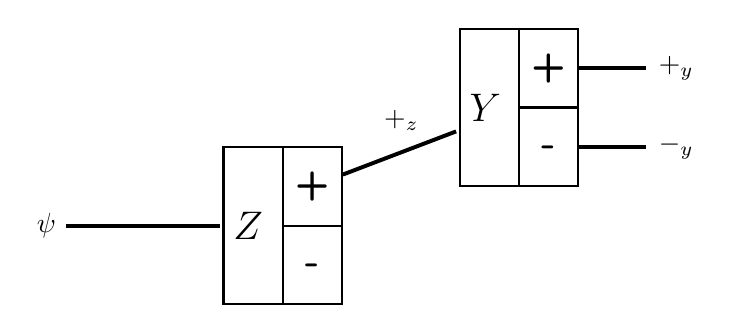
\begin{tikzpicture}[shorten >=1pt,auto, thick,
     square node/.style={rectangle, minimum height=2cm, minimum width=1.50cm, text width = 1.25cm, draw, font=\sffamily\Large\bfseries},
     port/.style={rectangle, draw,  minimum height=1cm, minimum width=0.75cm, font=\sffamily\Large\bfseries},
     wf/.style={rectangle, minimum height=1cm}]
    \apparatus{1}{3}{0}{$Z$};
    \apparatus{2}{6}{1.5}{$Y$};

    \node[wf] (w0) at (0,0) {$\ket{\psi}$};
    \node[wf] (w1) at (8, 2.0) {$\ket{+}_y$};
    \node[wf] (w2) at (8, 1.0) {$\ket{-}_y$};

    \draw[line width=0.5mm] (w0) -- (1);

    \draw[line width=0.5mm] (1+) -- (2) node [near end] {$\ket{+}_z$};

    \draw[line width=0.5mm] (2+) -- (w1);
    \draw[line width=0.5mm] (2-) -- (w2);
\end{tikzpicture}
\caption[Insert an abbreviated caption here to show in the List of Figures]
{Demonstrating renormalizing upon measurment in standard quantum mechanics}
\label{Figure:Measurement:Renormalizing}
\end{figure}

As an example, consider the system shown in \fref{Figure:Measurement:Renormalizing}. The first apparatus serves as a state preparation device, since we are only interested in particles exiting the spin-up output. Using the projection postulate, the state after the first measurement is
\begin{align}
    \ket{\psi_{top}} &= \frac{{P^z}_+\ket{\psi}}{\sqrt{\bra{\psi}{P^z}_+\ket{\psi}}} = \ket{+}_z
\end{align}
Similarly, the possible output states from the second apparatus are
\begin{align}
    \ket{\psi_{top}} &= \frac{{P^y}_+\ket{+}_z}{\sqrt{\tensor[_z]{\bra{+}}{}{P^y}_+\ket{+}_z}} = \ket{+}_y \\ \\
    \ket{\psi_{bottom}} &= \frac{{P^y}_-\ket{+}_z}{\sqrt{\tensor[_z]{\bra{+}}{}{P^y}_-\ket{+}_z}} = \ket{-}_y
\end{align}

TODO: carry out example calculations using Born rule

\section{Dynamics}
\invisiblesubsubsection{Postulate 6 (Unitary Dynamics)}
TODO: introduce 6th postulate (Schrodinger time evolution)

\chapter{Measurement}

TODO

\section{Measurement Problem}
Quantum mechanics is plagued by interpretational issues surrounding measurement. The state collapse mechanism described by the TODO REF fifth postulate occurs upon ``interaction with a classical measuring apparatus''. Lacking a precise definition of such an apparatus, the role of the experimentalist in measurement interactions is easily inflated. This ambiguity makes quantum mechanics exploitable for justification of anthropocentric worldviews, found in both popular and scientific literature:

\begin{quote}
``The human observer constitutes the final link in the chain of observational processes, and the properties of any atomic object can only be understood in terms of the object's interaction with the observer.'' \cite{Capra}
\end{quote}

\begin{quote}
``There exist external observers which cannot be treated within quantum mechanics, namely human (and perhaps animal) minds, which perform measurements on the brain causing wave function collapse.'' (Schreiber's description of the von Neumann–Wigner interpretation \cite{Schreiber})
\end{quote}

This attitude towards quantum measurement prompted Einstein to ask his colleague if he believed that the moon exists only when they looked at it \cite{Pais}. In this thesis, we assert that the moon does exist, even when not directly observed by a human. Instead, we allow a multitude of non-living systems to continuously ``measure'' the moon.

Furthermore, state collapse introduces dynamics entirely seperate from the unitary dynamics postulated by the Schrödinger equation. The dynamics to be employed depend upon whether or not the system is being ``measured''.

\section{von Neumann Measurement Scheme}

Using the \textit{von Neumann measurement scheme}, we describe the measurement interaction as a unitary physical process permitted by the Schrödinger equation. We no longer have to assume separate dynamics during measurement as a fundamental component of quantum theory.

To describe the apparatus as a quantum system, a \textit{pointer} Hilbert space is introduced to represent each measurement result. For a Stern-Gerlach apparatus, a pointer state is defined by the localization of the particle at spatially separated output regions. In general, a pointer state is some classical indicator; examples include an apparatus needle pointing up, or a particle colliding with a screen in a distinguishable region.

Let the pointer state space of the $z$ apparatus be represented by
\begin{align}
    {H^z}_\mathcal{X} = \{\alpha \ket{\mathcal{X}_+}_z + \beta \ket{\mathcal{X}_-}_z + \gamma \ket{\mathcal{X}_{ready}}_z\}
\end{align}
where $\alpha, \beta, \gamma \in \mathbb{C}$ and
\begin{align}
    _z\braket{\mathcal{X}_i|\mathcal{X}_j}_z&=\delta_{i,j}
\end{align}

Recalling the non-observability of superposition states TODO REF, we represent definite apparatus readings as pure pointer states. That is, $\ket{\mathcal{X}_+}_z$ represents the particle's localization in the spin-up region of the analyzer, $\ket{\mathcal{X}_-}_z$ the spin-down output region, and $\ket{\mathcal{X}_{ready}}_z$ anywhere else in space. These states are mutually exclusive (reflected by requiring orthonormality) and exhaustive (every position in space is encompassed by some pointer state). TODO REF addresses the question of the preferred basis problem.

We now consider $\ket{\psi}$ as the state of a composite spin-pointer system. We call our spin system $\ket{\psi}_s \in \mathcal{H}_s$, so that the composite state space is $\mathcal{H} = \mathcal{H}_s \otimes \mathcal{H}^z_\mathcal{X}$.

The von Neumann scheme describes measurement as \textit{entanglement} between pure pointer states and spin eigenstates. At the instant measurement begins $t_0$, the pointer state is $\ket{\mathcal{X}_{ready}}$ as the electron enters the magnetic field. At the instant measurement ends $t_1$, the pointer state is either $\ket{\mathcal{X}_{+}}$ or $\ket{\mathcal{X}_{-}}$, realized with spin-up and spin-down spin states respectively. This correlation is the desired result of unitary evolution.

Introducing the unitary operator that accomplishes this in explicit form,

\begin{align}
  U(t_0, t_1) = {P^z}_+ \otimes \left(\ket{\mathcal{X}_{+}}\bra{\mathcal{X}_{ready}} + \ket{\mathcal{X}_{ready}}\bra{\mathcal{X}_{+}} + \ket{\mathcal{X}_{-}}\bra{\mathcal{X}_{-}} \right) \\ \nonumber
  + {P^z}_- \otimes \left(\ket{\mathcal{X}_{-}}\bra{\mathcal{X}_{ready}} + \ket{\mathcal{X}_{ready}}\bra{\mathcal{X}_{-}} + \ket{\mathcal{X}_{+}}\bra{\mathcal{X}_{+}} \right)
\end{align}

In general, the final state is
\begin{align}
  U(t_0, t_1)\ket{\psi} & =  U(t_0, t_1) \left(\ket{\psi}_s \otimes \ket{\mathcal{X}_{null}}_z\right) \\
  &= {P^z}_+ \ket{\psi}_s \otimes \ket{\mathcal{X}_{+}}_z + {P^z}_- \ket{\psi}_s \otimes \ket{\mathcal{X}_{-}}_z
\end{align}

\begin{figure}
\centering\CaptionFontSize
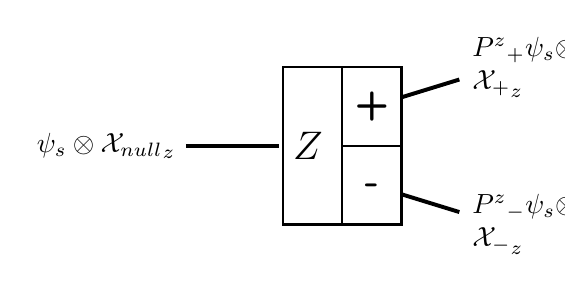
\begin{tikzpicture}[shorten >=1pt,auto, thick,
     square node/.style={rectangle, minimum height=2cm, minimum width=1.50cm, text width = 1.25cm, draw, font=\sffamily\Large\bfseries},
     port/.style={rectangle, draw,  minimum height=1cm, minimum width=0.75cm, font=\sffamily\Large\bfseries},
     wf/.style={rectangle, minimum height=1cm, text width = 0.7cm}]
    \apparatus{1}{3}{0}{$Z$};

    \node(w0) at (0,0) {$\ket{\psi}_s \otimes \ket{\mathcal{X}_{null}}_z$};
    \node[wf] (w1) at (5, 1.0) {${P^z}_+\ket{\psi}_s \otimes \ket{\mathcal{X}_+}_z$};
    \node[wf] (w2) at (5, -1.0) {${P^z}_-\ket{\psi}_s \otimes \ket{\mathcal{X}_-}_z$};

    \draw[line width=0.5mm] (w0) -- (1);
    \draw[line width=0.5mm] (1+) -- (w1);
    \draw[line width=0.5mm] (1-) -- (w2);
\end{tikzpicture}
\caption[Insert an abbreviated caption here to show in the List of Figures]
{Schematic Diagram of von Neumann Measurement}
\label{Figure:Measurement:DetectorStates}
\end{figure}

Notice that the final sum does not contain any terms representing incorrect correlations between spin and pointer states (such as $\ket{+}_s \otimes \ket{\mathcal{X_-}_z}$).  Consequently, the final state cannot be written as the tensor product of a state in $\mathcal{H}_s$ and a state in $\mathcal{H}^z_\mathcal{X}$ (as the inital state was). This is the definition of \textit{entanglement}; the von Neumann measurement scheme describes measurement as entanglement of the measured system and the apparatus.

In general, this process is described by a linear map:
\begin{align}
    \nonumber U(t_0, t_1): \\
    & \ket{\psi} = \left(\sum_{n} {P^z}_n\ket{\psi}_s\right) \otimes \ket{\mathcal{X}_{ready}}_z \mapsto \sum_{n}\left({P^z}_n\ket{\psi}_s \otimes \ket{\mathcal{X}_n}_z\right)
\end{align}

Notice that the initial state is a single tensor product, while the final state is a sum of tensor products. The coherence initially present only in the spin state is extended to the composite spin-pointer system. TODO: mention why this allows observation of quantum effects for multiple measurements.

By discarding the projection postulate, no notion of an undefined ``interaction with a classical apparatus'' is required to describe how states evolve when their properties are recorded. The various paradoxes and interpretational issues associated with state collapse are entirely circumvented.
